\documentclass[12pt]{article}
\usepackage{amsmath,amsthm,amssymb,dsfont,polynom}
\usepackage[pdftex]{graphicx}

\graphicspath{{images/}}

\usepackage{tikz}
\usetikzlibrary{arrows}

\usepackage[margin = 1.0in]{geometry}
\usepackage{fancyhdr}
\usepackage{hyperref}
\pagestyle{fancy}
\lhead{Francis Pich\'e}

\thispagestyle{empty}


\newtheorem{problem}{Problem} 
\theoremstyle{definition} 
\newtheorem*{solution}{Solution}

\usepackage{listings}
\usepackage{color}

\definecolor{dkgreen}{rgb}{0,0.6,0}
\definecolor{gray}{rgb}{0.5,0.5,0.5}
\definecolor{mauve}{rgb}{0.58,0,0.82}

\lstset{frame=tb,
  language= Python,
  aboveskip=3mm,
  belowskip=3mm,
  showstringspaces=false,
  columns=flexible,
  basicstyle={\small\ttfamily},
  numbers=none,
  numberstyle=\tiny\color{gray},
  keywordstyle=\color{blue},
  commentstyle=\color{dkgreen},
  stringstyle=\color{mauve},
  breaklines=true,
  breakatwhitespace=true,
  tabsize=3
}


\begin{document}
\title{COMP 557 Study guide}
\author{Francis Pich\'e}
\date{\today}
\maketitle
\newpage
\tableofcontents
\newpage

\part{Introduction}
\section{Disclaimer}
These notes are curated from Professor Paul Kry COMP557 lectures at McGill University. They are for study purposes only. They are not to be used for monetary gain.
\section{About This Guide}
I make my notes freely available for other students as a way to stay accountable for taking good notes. If you spot anything incorrect or unclear, don't hesitate to contact me via Facebook or e-mail at \url{http://francispiche.ca/contact/}
\part{Transformations}
\section{Notation}
\subsection{Implicit Representation}
$$(1)\{\vec{v}|f(\vec{v}) = 0\}$$
In English, this means the set of all vectors $v$, such that some function $f$ of $v$ gives zero. For example, if $f = \vec{v}\cdot\vec{u} + k$. Then the set of all vectors which satisfy $(1)$ would be some line (since the dot product gives a scalar, and the $k$ is a scalar. So we need to dot product to be $-k$). If $k$ is 0, then the set is just the set of vectors orthogonal to $\vec{u}$, which is a line.
\\ \linebreak
Another example: $$\{\vec{v} | (\vec{v} - \vec{p})\cdot(\vec{v} - \vec{p}) - \vec{r}^2 = 0 \}$$
This is just a fancy way of expressing the equation of a circle centered at $\vec{p}$. (Plug some sample vectors in if you don't believe it)
\subsection{Explicit (Parametric) Representation}
A parameter is given with a specified domain to describe the equation. For example: $$\{\vec{p} + r\begin{pmatrix}
cos(t) \\ sin(t)
\end{pmatrix} | t \in [0,2\pi]\}$$ describes a circle.
\section{Linear Transformations}
A great video (and series) to visualize the linear algebra used in graphics is \href{https://www.youtube.com/watch?v=kYB8IZa5AuE}{this from 3Blue1Brown} on YouTube.
\\ \linebreak 
Transformations are like "functions" that operate on a set of points. 
\\ \linebreak
Parametric form of a mapping from one set to another using some transform $T$:
$$ \{f(t) | t \in D\} \rightarrow \{T(f(t))|t \in D\}$$
Implicit form:
$$\{ \vec{v}| f(\vec{v} = 0)\} \rightarrow \{T(\vec{v})| f(\vec{v}) = 0\}$$
$$ = \{\vec{v} | f(T^{-1}(\vec{v})) = 0\}$$
To convince yourself of that last equality, try it on few examples.
\\ \linebreak
Translation: $$T(\vec{v}) = \vec{v} + \vec{u}$$
\\ \linebreak
See the slides for visual representations of the common linear transformations: (translation, sheer, scale, rotation, reflection etc.) The video mentioned above is also nice for getting a feel of how it works.
\subsection{Combining Linear Transforms with Translation}
Could do it this way:
$$T(\vec{p}) = M\vec{p} + \vec{u}$$
for some matrix $M$, but if you try to do that with a composition:
$$T(\vec{p}) = M_T\vec{p} + \vec{u}_T$$
$$S(\vec{p}) = M_S\vec{p} + \vec{u}_S$$
then
$$(S \circ T) = M_S(M_T\vec{p} + \vec{u}_T) +\vec{u}_S$$
which is honestly pretty gross to look at. We can do better using $homogeneous$ $coordinates$. 
\subsubsection{Homogeneous Coordinates}
This is the use of a 3x3 matrix to perform translation with a linear transformation. We add an extra component $w$, to our 2x2 vectors, and an extra row $(0, 0 ,w)$ and column $\begin{pmatrix} 0 \\ 0 \\ w\end{pmatrix}$
For points in an affine space, $w=1$. 
\\ \linebreak
Linear transformations:
$$\begin{pmatrix}
a && b && 0 \\
c && d && 0 \\
0 && 0 && 1 \\
\end{pmatrix}
\begin{pmatrix}
x \\ y \\ 1
\end{pmatrix} =
\begin{pmatrix}
ax + by \\
cx + dy \\
1
\end{pmatrix}$$
Translation (uses the extra column):

$$\begin{pmatrix}
	1 && 0 && t \\
	0 && 1 && s \\
	0 && 0 && 1 \\
\end{pmatrix}
\begin{pmatrix}
	x \\ y \\ 1
\end{pmatrix} =
\begin{pmatrix}
	x + t \\
	y + s \\
	1
\end{pmatrix}$$
If we now do composition, we can do it like this (using block notation):
$$
\begin{pmatrix}
M_S && \vec{u}_S \\
0 && 1
\end{pmatrix}
\begin{pmatrix}
M_T && \vec{u_T} \\
0 && 1
\end{pmatrix}
\begin{pmatrix}
p \\ 1
\end{pmatrix}$$
$$
= \begin{pmatrix}
M_SM_T && M_S\vec{u_T} + \vec{u_S} \\
0 && 1
\end{pmatrix}
\begin{pmatrix}
p \\
1
\end{pmatrix}
$$
Which is essentially the same, but cleaner and will be more useful later.

\subsection{Affine Transformations}
These are transformations in which lines that were straight, and lines that were parallel to each other are still straight and parallel to each other. Also, the ratios of lengths along lines are preserved.
\\ \linebreak
Common transforms:
\\ \linebreak
Translation:
$$\begin{pmatrix}
1 && 0 && t_x \\
0 && 1 && t_y \\
0 && 0 && 1
\end{pmatrix}$$
is a translation of $t_x$ in the $x$ direction and $t_y$ in the $y$.
\\ \linebreak
Scale:
$$\begin{pmatrix}
s_x && 0 && 0 \\
0 && s_y && 0 \\
0 && 0 && 1
\end{pmatrix}$$
to scale $s_x$ in the $x$-axis and $s_y$ in the $y$-axis.

\subsection{Rigid Motions}
A transformation made up of only translation and rotation is a rigid motion.
\\ \linebreak
Note that for rotations, the inverse is the transpose (rotation matrices are orthogonal), and so the inverse of a rigid motion $E$ is:
$$ E = \begin{pmatrix}
R && \vec{u} \\
0 && 1
\end{pmatrix}
$$
$$
E^{-1} = \begin{pmatrix}
R^T && -R^T \vec{u} \\
0 && 1
\end{pmatrix}
$$
\subsection{Composing to change axes}
To rotate about a point other than the origin, first we translate, then rotate, and translate back.
$$M = T^{-1}RT $$
To scale along a particular axis and point, you would move it to the point, rotate so that the axis lines up with the x or y axis, scale, then undo all the operations.
$$M = T^{-1}R^{-1}SRT$$

\subsection{Points vs. Vectors}
Points and vectors are NOT the same. Points are locations in space, whereas vectors can be thought of displacements in space, or a tuple of distance and direction between points.
\\ \linebreak
In homogeneous coordinates, vectors have $w=0$. 
\\ \linebreak
Translations do not affect vectors:
$$\begin{pmatrix}
M && t \\
0 && 1 
\end{pmatrix}
\begin{pmatrix}
p \\ 1
\end{pmatrix}
= \begin{pmatrix}
Mp + t \\ 1
\end{pmatrix}$$
$$
\begin{pmatrix}
M && t \\
0 && 1
\end{pmatrix}
\begin{pmatrix}
v \\ 0
\end{pmatrix}
=
\begin{pmatrix}
Mv \\ 0
\end{pmatrix}$$
\section{Change of Coordinates}
This is similar to the idea of moving an object to the origin to apply transformations and moving it back, but more formulaic. (A computer could do it!)
\\ \linebreak
$$T_e = FT_FF^{-1}$$
Where $T_e$ is the transform expressed with respect to the canonical basis (The form we're used to). $T_F$ is the transformation expressed in the $natural$ frame. $F$ is the transform which takes us from the new basis to the canonical one. It's form is: $\begin{pmatrix}\vec{u} && \vec{v} && \vec{p}\end{pmatrix}$ where u, v are the axes and p is the new origin.
\\ \linebreak
\section{Aside: Classes of transforms}
There is a sort of "hierarchy" of transforms. The classes are as follows:
\begin{itemize}
	\item Homographies (Lines remain lines)
	\item Affine (preserve parallel lines)
	\item Conformal (Also preserve angles)
	\item Rigid (also preserve lengths)
\end{itemize}
where: $$ Rigid \subseteq Conformal \subseteq Affine \subseteq Homographies$$

\section{3D Transformations}
3D Transformations are essentially the same as 2D. (where we add the extra row/column and put a 1 or 0) We simply use a 4x4 matrix instead of a 3x3. For example:

$$\begin{pmatrix}
x' \\ y' \\ z' \\ 1
\end{pmatrix}=
\begin{pmatrix}
1 && 0 && 0 && t_x \\
0 && 1 && 0 && t_y \\
0 && 0 && 1 && t_z \\
0 && 0 && 0 && 1
\end{pmatrix}
\begin{pmatrix}
	x \\ y \\ z \\ 1
\end{pmatrix}$$
Would be a translation by $t_x$ ,$t_y$ and $t_z$. 
\\ \linebreak
Rotations get a little weird. We not only have to specify an angle, but now also an axis of rotation. So:
$$\begin{pmatrix}
x' \\ y' \\ z' \\ 1
\end{pmatrix}=
\begin{pmatrix}
cos(\theta) && -sin(\theta) && 0 && 0 \\
sin(\theta) && cos(\theta)  && 0 && 0 \\
0           && 0            && 1 && 0 \\
0           && 0            && 0 && 1
\end{pmatrix}
\begin{pmatrix}
x \\ y \\ z \\ 1
\end{pmatrix}$$
Would be a rotation about the $z$ axis.
$$\begin{pmatrix}
x' \\ y' \\ z' \\ 1
\end{pmatrix}=
\begin{pmatrix}
1 && 0            && 0           && 0 \\
0 && cos(\theta)  && -sin(\theta)&& 0 \\
0 && sin(\theta   && cos(\theta) && 0 \\
0 && 0            && 0           && 1
\end{pmatrix}
\begin{pmatrix}
x \\ y \\ z \\ 1
\end{pmatrix}$$
Would be a rotation about the $x$ axis.
\\ \linebreak
As you can see, this is pretty messy to come up with for an arbitrary axis. It would be nice to represent rotations in more intuitive ways.
\\ \linebreak
A matrix for a reflection in the plane which passes through the origin, with normal $n$ would be derived as follows. First, we need to project the point $p$ onto the normal $n$, using the dot product $$(n \cdot p)n$$. (You can imagine the dot was moved onto the normal line) Then multiplying by -2 to move the dot through the plane backwards: $$-2(n \cdot p)n$$ We now move the dot to where it should float in space by adding $p$. $$-2(n \cdot p) + p$$
To now express this as a matrix, we use $n$ and $p$ as vectors, and add $Ip$ at the end instead of $p$. $$ p' = -2 (\begin{pmatrix}
	n_x \\ n_y \\ n_z
\end{pmatrix}
\begin{pmatrix}
	n_x && n_y && n_z
\end{pmatrix}) +
\begin{pmatrix}
	1 && 0 && 0 \\
	0 && 1 && 0 \\
	0 && 0 && 1
\end{pmatrix}
\begin{pmatrix}
	p_x \\ p_y \\ p_z
\end{pmatrix}
$$
\subsection{Rotations in 3D}
In general, 3D scaling, rotation and translation do not commute. Think of a rotation followed by a non-uniform scale. This will appear to mutate the object. See (\url{https://www.youtube.com/watch?v=ThD1h-0_noE} for an illustration) The reason is that the axis of scaling changes before the scale is applied.
\\ \linebreak
Similarly, a translation followed by a rotation does not commute. The axis of rotation will be relative to the origin, but we're no longer at the origin, so the object would move in a wide arc around the origin rather than rotate around it's center as we'd expect.
\\ \linebreak
Note that 3D rotations are defined as:
$$ R \in \mathds{R}^{3x3}: R^T = R^{-1}, det(R) = 1$$
Also note that we have 3 more degrees of freedom in 3D, since we can rotate about any axis. So knowing the angle, and the axis direction is all the info required to describe a rotation.
\subsection{Euler Angles}
Coming up with general rotation matrices is kind of hard, so it can be useful to break them down into rotations about the canonical axes. This is possible with Euler Angles.
\\ \linebreak
Any rotation can be broken down into 3 rotations about the $x$, $y$, or $z$ axis.
\\ \linebreak
The first rotation is rotating in the canonical frame, while the others are rotating with respect to the object frame. 
\\ \linebreak
It takes exactly 3 rotations, with no two successive rotations being along the same axis to be able to express ANY rotation. (Euler's Theorem)
\\ \linebreak
\subsubsection{Gimbal Lock}
This is a problem that can occur with using Euler Angles if the first rotation "squashes" an axis. That is, the rotation places the new axis directly on top on an existing axis, removing a possible axis of rotation. 
\\ \linebreak
For example a rotation of 90 degrees about the $z$ axis would leave the $z$ on top of the $x$, removing the possibility of rotating about the $z$ and $x$ axes independently.
\\ \linebreak
This video that Prof. Kry put in the slides is super useful for understanding Euler angles and Gimbal lock. \url{https://www.youtube.com/watch?v=zc8b2Jo7mno}

\subsubsection{Interpolation of Euler Angles}
If you simply interpolate each rotation one after the other, you'll get different paths for different orders of rotation. For example if you rotate $xyx$ you'd get a different path than $xyz$ even if the end rotation is the same. Changing the order of rotations can also be leveraged to avoid Gimbal lock.

\section{Scene Graphs}
When you have multiple objects in a scene, and need them to have working relationships in terms of how they move, we use a scene graph. 
\\ \linebreak
This allows for the grouping of objects in a way that makes sense. For example, you can (as in the assignment) make a character with limbs that can move independently, or together depending on where you apply transformations in the graph.
\\ \linebreak
In general, we use a "group" node to keep sets of objects together. Interior nodes in the graph are groups, and the leaves are objects.
\\ \linebreak
However, we can also have relations to multiple "parents" so we actually have a directed acyclic graph, not a tree (DAG).

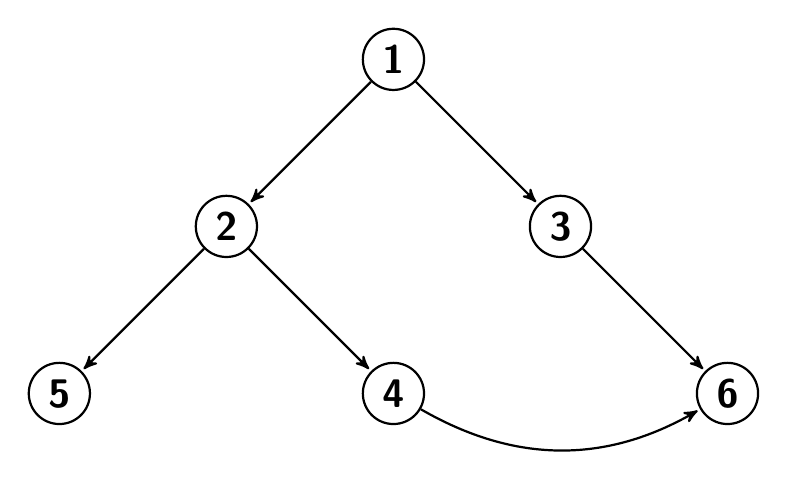
\begin{tikzpicture}[->,>=stealth',shorten >=1pt,auto,node distance=3cm,
thick,main node/.style={circle,draw,font=\sffamily\Large\bfseries}]
	
	\node[main node] (1) {1};
	\node[main node] (2) [below left of=1] {2};
	\node[main node] (3) [below right of=1] {3};
	\node[main node] (4) [below right of=2] {4};
	\node[main node] (5) [below left of=2]{5};
	\node[main node] (6) [below right of=3]{6};
	
	\path[every node/.style={font=\sffamily\small}]
	
	(1) edge node [right] {}(3)
		edge node [left] {}(2)
	
	(2) edge node [right] {}(4)
		edge node [left] {}(5)
		
	(3) edge node [right] {}(6)
	
	(4) edge [bend right] node [right] {}(6);
	
\end{tikzpicture}
\\
So here, tranforming 1 will apply the same transform to all the nodes, whereas transforming 3 or 4 will affect 6, and transforming 6 will affect only 6. 
\\ \linebreak
Having multiple parents is called "instancing".
\\ \linebreak
Object orientation is useful since we can naturally implement a hierarchy with the \texttt{extends} relationship.

\subsection{Transforms on the Graph}
Transforms accumulate from the root (ie the leaves are the leftmost matrices, the root is on the right)
\\ \linebreak
Traversal in OpenGL is done by keeping a matrix stack. We can keep sub-trees separate conceptually by creating matrices for each sub-tree and adding it to the stack. We then pop it when we're done.
\\ \linebreak
We often want to group nodes by adding an identity node as a parent, or ungroup notes by pushing the transform of the parent to the children.
\\ \linebreak
We can also re-parent by moving a node from 
\section{Quaternions}
Like complex numbers but with more dimensions:
$$ ijk = i^2 = j^2 = k^2 = -1$$
They are manipulated similarly to complex numbers.
$$A = a_0 + a_1i + a_2j + a_3k$$
$$B = b_0 + b_1i + b_2j + b_3k$$
$$AB = a_0b_0 - a_1b_1 - a_2b_2 - a_3b_3 + (a_0b_1 + a_1b_0 + a_2b_3 + a_2b_3 - a_3b_2)i ...$$
Quaternions can be used to represent rotations!
\\ \linebreak
It represents a rotation by an angle $\theta$ along an axis $(x, y, z)$. $$q = (c, sx, sy, sz) \equiv c + sxi + syj + szk$$ where $c = cos(\theta/2)$ and $s = sin(\theta/2)$. It's $\theta/2$ because $q$ and $-q$ are exactly the same rotation! 

\section{Considerations For Choosing Rotations}
There are many considerations for choosing what kind of rotation specification we want. For example, we may want to avoid euler angles if Gimbal lock is a problem, or we may prefer the interpolation of one over another.
\\ \linebreak
\begin{itemize}
	\item Numerical issues (matrix multiplication may get messed up)
	\item Space (matrices use more memory than vectors etc)
	\item Conversions (converting from a matrix to Euler angles is hard etc)
	\item Speed (Composing for points is faster with Quaternions, but for 		vectors is slower)
	
\end{itemize}

\subsection{Linear Interpolation}
To linearly interpolate (or $Lerp$) between two points $a$ and $b$:
$$ Lerp(t, a, b) = (1-t)a + (t)b$$
where $0\leq t \leq1$.
\\ \linebreak
Notice that $Lerp$ with Euler angles is going to move in different directions before getting to the final destination, while a quaternion or single matrix will do it in one smooth motion.
\\ \linebreak
Spherical linear interpolation is given by:
$$Slerp(t, a, b) = \frac{sin((1-t)\theta)}{sin(\theta)}a + \frac{sin(t\theta)}{sin(\theta)}b$$
where $ \theta = cos^{-1}(a\cdot b)$  \\ \linebreak
This is used for smoothly interpolating two rotations given by a quaternion. But be careful! If $a \cdot b$ is negative, the direction of rotation changes, and since for quaternions the negative is the same rotation, you get two different interpolations for the same angle!

\section{Building Rotations}
If we wanted to build some arbitrary rotation matrix, we could just compose it with elementary transforms, (multiply by some translation $T$ and rotation $R$ so that the rotation axis we want to rotate by is aligned with the x-axis.) then apply the rotation, and move everything back. In 3-D, you would need to:
\begin{itemize}
	\item Translate rotation axis to pass through the origin
	\item Rotate about y to align the object with the x-y plane
	\item Rotate about the z axis so that the axis we want to rotate by is along the x. 
\end{itemize}

We could also just construct a change of coordinates: 
$$T = FR_X(\theta)F^{-1}$$ 
where $$F = \begin{pmatrix}
u && v && w && p \\
0 && 0 && 0 && 1
\end{pmatrix}$$
Where $p$ is a point the axis of rotation run through, and $u$, $v$ and $w$ are chosen as follows:
\\ \linebreak
If you have two vectors, $a$ and $b$, you can take:
$$ u = \frac{u}{||u||}$$
$$ w = u x b $$
$$ v = w x u $$ 
where $u$ matches the rotation axis, and $p$ is a point along $u$.
\\ \linebreak
We count our degrees of freedom in a transformation by counting the number of matrix elements we can change. For example:
$$\begin{pmatrix}
	a && b && c && d \\
	e && f && g && h \\
	i && j && k && l \\
	0 && 0 && 0 && w \\
\end{pmatrix}$$
We can't change $w$ or the zero's so we have 12 degrees of freedom in 3D.
\section{Transforming Normal Vectors}
Normals are vectors that are perpendicular to the object surface. They are covectors (not differences between points!) so they can get messed up by non-uniform scales and sheers (but not rotations or rotations!)
\\ \linebreak
To "fix" them you will need to use $$X = (M^T)^{-1}$$ where $M$ is the transformation matrix on the object. This is because: $$Mt \cdot Xn = t^TM^TXn$$
$$= t^TM^T(M^T)^{-1}n = t^Tn = 0$$
Where $t$ is a vector tangent to the surface and $n$ is the normal.
\\ \linebreak


\part{Viewing and Projection}
\section{Image Order and Object Order}
With image order, the scene is generated by calculating rays coming from the eye, through each pixel on the screen and calculating how rays of light would interact with the objects. This is known as \textit{ray tracing}.
\\ \linebreak
In contrast, \textbf{Object order} viewing is when we take points on the object and project them onto a 2 plane (the screen). 
\section{Camera Transformation}
When dealing with viewing, we always talk about the eye as the origin, and we always "look" down the $z$ axis. 
\\ \linebreak

\subsection{Lookat Transformation}
We want to find a transformation that will put our view to look at a specific point. 
\\ \linebreak
We do this by computing a transform from points: 
\begin{itemize}
\item $e$ the eye point
\item $l$ the lookat point
\item $v_{up}$ to know which way is up.
\end{itemize}
We do this by first rotating by some matrix $R$, then translating by $T$.
\\ \linebreak
Similar to how we did 3D transformations, we need a matrix:
$$\begin{pmatrix}
u && v && w && e \\
0 && 0 && 0 && 1
\end{pmatrix}^{-1}$$
$w$ is a vector pointing in the opposite direction of the direction we want to look, so 
$$ w = \frac{l-e}{||l-e||}$$
To get $v$, we project $v_{up}$ onto the plane perpendicular to $w$.
$$v = v_{up} - (v_{up} \cdot w)w$$
Then lastly we want $u$ to by perpendicular to both so :
$$ u = v \text{x} w$$
I'll be honest I had to review projections to understand this, but I really recommend it!
\\ \linebreak
Now we can apply the transformation as a change of basis like we do normally.
\\ \linebreak
\section{Orthographic Projection}
In graphics, we specify a near plane, and a far plane. The near plane is what we are going to see, and it lies in front of the center of projection (the eye).
\\ \linebreak
In orthographic projection, we simply remove the $z$ axis. 
\\ \linebreak
$$ \begin{pmatrix}
x' \\ y' \\ z'
\end{pmatrix} =
\begin{pmatrix}
x \\ y \\ z
\end{pmatrix}
\begin{pmatrix}
1 && 0 && 0 && 0 \\
0 && 1 && 0 && 0 \\
0 && 0 && 0 && 1 \\
\end{pmatrix}
\begin{pmatrix}
x \\ y \\ z \\ 1
\end{pmatrix}$$
\subsection{Orthographic Viewport Transformation}
To be able to put the image on the screen, we need to think in terms of pixel units. So if our view is $x$ by $y$, we have $n_x$ by $n_y$ pixels, where each pixel has size $2/n_x$ by $2/n_y$
\\ \linebreak
The transformation is then:
$$\begin{pmatrix}
x_{canonical} \\
y_{canonical} \\
\end{pmatrix}
\begin{pmatrix}
\frac{n_x}{2} && 0 &&\frac{n_x-1}{2} \\
0             && \frac{n_y}{2} && \frac{n_y-1}{2} \\
0 && 0 && 1
\end{pmatrix}
=
\begin{pmatrix}
x_{screen} \\ y_{screen} \\ 1
\end{pmatrix}
$$
Now, we need to specify a viewing volume. That is, some planes that restrict what we'll be seeing, to set limits for the rendering. All we need to specify is a near, $n$, far $f$, left $l$ and right $r$.
\\ \linebreak
This is a 3D windowing transformation, so:
$$\begin{pmatrix}
\frac{2}{r-l} && 0 && 0 && -\frac{r+l}{r-l} \\
0 && \frac{2}{t-b} && 0 && -\frac{t+b}{t-b} \\
0 && 0 && \frac{2}{n-f} && -\frac{n+f}{n-f} \\
0 && 0 && 0 && 1
\end{pmatrix}$$

\section{Planar Perspective Projection}
To implement perspective, points that are further away need to be proportionally "shrunk". This is done as follows:
\\ \linebreak
If $d$ is the distance down the $-z$ direction, and $y$ is the height of an object, then:
$$\frac{y'}{d} = \frac{y}{z}$$
Were $d$ is the distance to the plane that we're projecting onto, $y'$ is the shortened height, and $y,z$ are the coordinates of the original object.
\\ \linebreak

We can do this due to similar triangles, and this means that $$y' = -dy/z$$
\subsection{Homogeneous Coordinates Revisited}
Recall that points in 3d can be represented as:
$$\begin{pmatrix}
wx \\ wy \\ wz \\ w
\end{pmatrix}$$
For $w \neq 0$. But now think if $w$ was arbitrarily close to 0, we would be scaling the points so far that it would be a point at infinity. This could be the point at which parallel line intersect.
\\ \linebreak
With perspective projection, we put $-z$ into $w$. Using the similar triangles fact from before, we know
$$\begin{pmatrix}
-dx/z \\ -dy/z \\ 1
\end{pmatrix}~\begin{pmatrix}
dx \\ dy \\-z
\end{pmatrix}$$
So then 
\subsection{Carrying Depth Through Perspective}
Doing perspective projection like above is fine, but we lose all information about the original depth! (Since we're projecting onto a flat plane). We need some way to maintain this information, so that we can know which objects are supposed to be "in front" of other objects.
\\ \linebreak
We can do this by adding some special $a$ and $b$ to our matrix. 
$$\begin{pmatrix}
n && 0 && 0 && 0 \\
0 && n && 0 && 0 \\
0 && 0 && a && b \\
0 && 0 && -1 && 0 \\
\end{pmatrix}$$
Where we choose $a$ and $b$ such that: $z'(-n) = -n$ and $z'(-f) = -f$ \\ \linebreak
It turns out that:
$$a = n =f $$, 
$$nf = b$$.
See slide 35 of the Projection slides for the derivation.
\\ \linebreak
Using this, we can see that:
\begin{itemize}
	\item Lines through the origin become parallel
	\item Vectors map to the plane: $z = n + f$ 
	\item Points on a plane with a z-normal which runs throuh the center of projection get mapped to points at infinity.
	\item Points halfway between the near and far plane get mapped to a point where $z$ 
	\item  Points behind the camera get mapped beyond the $n + f$ plane, and the x, y coordinates get reflected.
	
\end{itemize}
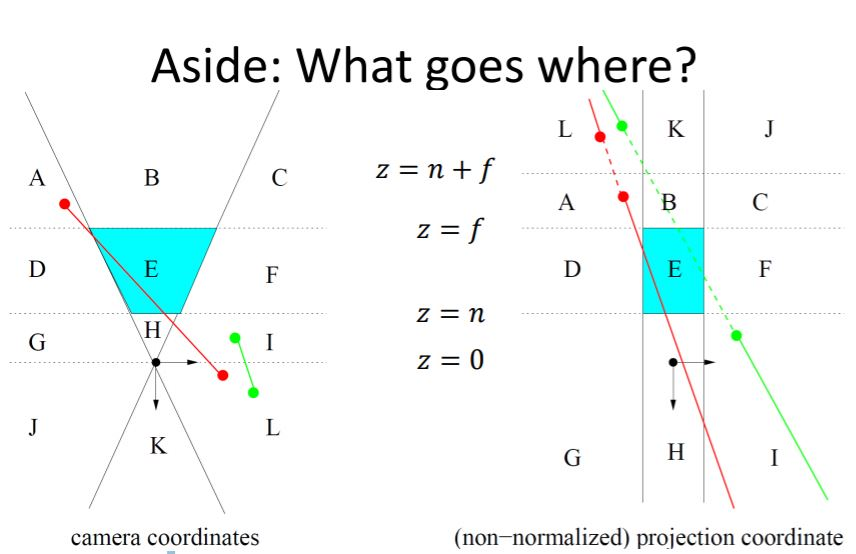
\includegraphics{what_goes_where}
\\ \textit{Figure 1. Paul Kry 3D Viewing, Orthographic and Perspective Projection slide \#37}\\ \linebreak
We can then use the orthographic windowing transform, combined with our projection matrix to get the full projection and window;
$$M_{per} = M_{orth}P$$ 
Where $P$ is the perspective projection.
\\ \linebreak

\subsection{OpenGL Transformation Pipeline}
In OpenGL, the position on the screen, $p_s$ of a point in the world $p_o$ is given by the following transformations:
$$M_{vp}M_{orth}PM_{cam}M_mp_o$$
Or (from right to left) the point, times the modelview matrix, times the camera transformation (the transform into camera coordinates, aka lookat), times the perspective matrix, times the orthogonal projection matrix, times the viewport matrix.
\\ \linebreak
In open GL, this breaks down into 3 matrices. $M_{cam}M_M$ is the \texttt{GL\_MODELVIEW\_MATRIX}, $M_{orth}P$ is the \texttt{GL\_PROJECTION\_MATRIX} and the viewport is by itself.

\subsection{Frustum Applications}
As done in assignment 2, we can implement different frustums to achieve different effects. For example, depth of field can be achieved by overlaying multiple views from shifted perspectives, such that the focal plane is the point of intersection of all the frustums. Or we can make 3D anaglyphs by using two shifted eye positions. 
\\ \linebreak
EVERYTHING IS WITH SIMILAR TRIANGLES. That's it. There are no other tricks. It's all about drawing the correct picture and choosing the correct triangles. See slides 51-53 on the Viewing slide deck for some really useful pictures.

\section{Projection Taxonomy}
Projections can be broken down in to classes depending on behavior. Names are assigned to be able to describe them precisely, like biologists with their kingdoms, classes, families and species.
\\ \linebreak
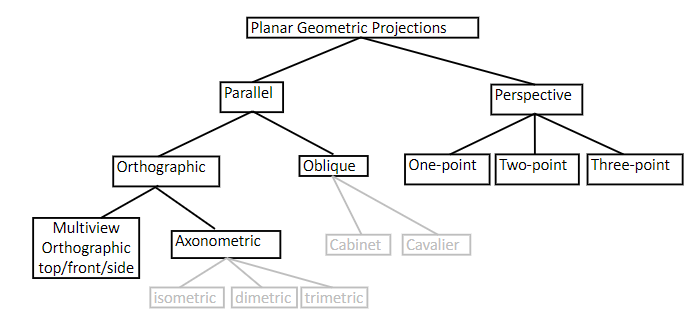
\includegraphics{taxonomy}
\\ \textit{Figure 2. Paul Kry 3D Projection Taxonomy slide \#3}

\subsection{Parallel Projection}
Parallel projection is when the viewing rays are parallel. So instead of having an eye from which there is a field of view and rays would come out in a sort of arc, all rays come straight out and parallel.

\subsubsection{Orthographic}
Orthographic projection breaks down into \textbf{mulitview} and \textbf{axonometric}. 
\\ \linebreak
Multiview is when the projection plane is parallel to some coordinate plane. Ie: Looking directly down the x, y, or z axis.
\\ \linebreak
Axonometric is an off-axis parallel projection. This splits into trimetric, dimetric, and isometric. The difference between them is the number of viewing axes that are equally forshortened, with isometric at all, and trimetric at none.

\subsubsection{Oblique}
Oblique projection is when the projection plane is parallel to a coordinate plane, but not parallel to a projection direction. This breaks down into cabinet(half length in z) and cavalier (same length in all directions).

\subsection{Perspective}
This breaks down into one point, two point and three point perspective, where the difference is the number of axis that are affected by the perspective projection.
\\ \linebreak
The field of view will determine the "strength" of the perspective effect. For example, a close viewpoint with wide angle would cause strong foreshortening, while a far viewpoint with narrow angle would cause very little.
\subsubsection{Shifted Perspective}
This is when the projection plane is not perpendicular to the view direction. ie) if you had a focal plane which was tilted, or an eye position that was off-center but still looking at the same rectangle than if it wasn't shifted (like the assignment).
\\ \linebreak
This allows for more control over the convergence of parallel lines. For example, if you look straight at a building, the top will be the same size as the bottom, but if you look up (tilt the viewing frame) the top will seem smaller.

\section{Field of View}
This is the angle between the opposite edges of a perspective image. That is, if you look at the shape of the frustum, the angle between the the top/bottom of the view volume, or the left/right. The field of view can have interesting effects on the "strength" of a perspective effect (similar to the close/far viewpoint). Having a narrow angle will cause a "flattening" whereas a wider angle will cause a "deeper" perspective.

\part{Lighting and Pipeline}

\section{Shading Overview}
In shading, we compute how light would be reflected/scattered from a light source, to a camera. To do this, we need:
\begin{itemize}
	\item Eye direction
	\item Light direction
	\item Normal of the surface
	\item Properties of the surface
\end{itemize}
In general, how much light an area receives is proportional to the cosine of the angle between the normal of the surface, $n$ and the direction of the light $l$. So it makes sense to express with a dot product. $l \cdot n$\\ \linebreak

\section{Lambertian Shading}
Here, we assume that light is scattered equally in all directions. The resulting light is computed by the following equation:
$$L_d = k_dImax(0, n\cdot l)$$
where $k_d$ is some constant related to the properties of the surface, and $I$ is the intensity of the light.
\\ \linebreak
Each color channel is processed separately. In this sense, you could think of$k_d$ and $I$ as 3-tuples of colors, and their product would be a component-wise product.
\\ \linebreak
\textbf{Lambertian Shading makes a matte effect}

\section{Specular Shading}
\subsection{Phong Model}
In the Phong model, the resulting light intensity depends on the view direction. The smaller the angle between the eye and the vector which lies at 90 degrees from the light source, the brighter the result.

$$L_s = k_sImax(0, r\cdot v)^p$$
where $k_s$ is some specular coefficient for the surface, $p$ is the shininess, $r$ is orthogonal to the light, and $v$ is the viewing direction.
\\ \linebreak
$r$ is computed as follows:
$$r = n(n\cdot l) - (I - n\cot n^T)l$$
$$ = (2nn^T - I)l$$
The first equation comes from projecting $l$ on to $n$, then the second portion is $n$ onto $l$, taking into account the intensity, $I$. The result is a vector which mirrors initial light.
\\ \linebreak
The Phong model is not based on physics, and thus is prone to some anomalies. (notably when the camera is behind the light, it suddenly clamps (because of the max(0, x)).

\subsection{Blinn-Phong Model}
The Blinn-Phong model uses the half vector between $l$ and $v$ instead of the true reflection of $l$. It is thus cheaper to compute.
$$L_s = k_sIMax(0, n\cdot h)^p$$. where $$h= \frac{v + l}{|v+l|}$$

\section{Ambient Shading}
The light which does not depend on a specific light source (ie: everything is a light source) is simply computed by:
$$ L_a = k_aI_a$$ 

\section{Lighting All Together}
The light in any given spot is usually just the sum of the diffuse light, specular light, and ambient light. 
$$L = L_a + L_d + L_s$$
$$ = k_aI_a + k_dImax(0, l\cdot v) + k_sImax(0, l\cdot h)^p$$
If we had many lights, we simply sum all of the diffuse and specular lights, adding the ambient at the end only once.
\\ \linebreak

\section{Hidden Surface Elimination}
How can we ensure that we do not draw surfaces that are occluded by others?
\subsection{Back Face Culling}
You could only draw faces that are facing the camera, by going around the object counter clockwise and any face which runs downward, and only draw that. 
\\ \linebreak
\subsection{Painters algorithm}
While this doesn't always work in more complex cases, we can simply draw our objects back to front, and ignore any overlaps. This works well if no objects are behind one, but also in front of another object (interleaved), and when we have information about the z coordinate of all objects (with respect to the eye).
\subsection{Warnocks Algorithm}
This is an algorithm which extends the Painters algorithm by subdividing the surface and applying the Painters algorithm when it can.
\subsection{Z Buffer}
Maintaining and sorting a Z ordering of objects is expensive. If the view changes, the entire thing must be recomputed. 
\\ \linebreak
The solution is to draw the objects in any random order, and just keeping track of that the closest object is. Each pixel then stores what the closest object is so far, and then, when drawing, compare the objects depth to this "closest" depth.
\\ \linebreak
The issue with this is that an equally spaced set of z points in the perspective is not necessarily equally spaced in the eyes point of view. (Remember how the perspective projection distorts points). Therefore we cannot simply linearly interpolate them and expect to be the same. 
\\ \linebreak
Things closer to the near plane can be more precise, while with things near the far plane, the unit distances in world coordinates start to become very far in eye coordinates, so we lose precision.

\section{Infinite Viewing/Light}
Since most lighting requires geometric information about the light vector, eye vector and surface normal, and the light and eye vectors constantly change, we would have to do a lot of recomputation.
\\ \linebreak
If we can approximate values by assuming that the eye and light are infinitely far away, we do not need to constantly recompute the lighting.
\\ \linebreak

\part{Meshes}
\section{Definitions}
\textit{Manifold}: Topological space that locally represents a plane. ie: can lay out a pizza onto/over it.
\\ \linebreak
\textit{Boundary} If an edge only belongs to one polygon\\ \linebreak
\textit{Front face} counter clockwise ordering of edges.\\ \linebreak
\textit{Compatible}, two faces are compatible the shared faces are in opposite order.\\ \linebreak
\textit{Orientable} if all adjacent faces are compatible.
\\ \linebreak
Example of a non-orientable manifold: mobius strip.
\\ \linebreak
\textit{Polyhedron:} Closed orientable manifold which makes up a volume.
\\ \linebreak
\textit{Genus} The number of "handles" or spaces where you could cut it and still have a connected manifold.\\ \linebreak
\textit{Euler Characteristic}: 
$$ V - E + F + 2g + \#\delta = 2$$
Number of vertices minus edges plus faces plus twice the genus plus the number of boundaries = 2.
\\ \linebreak
\textit{Topological Validity}: be manifold.
\\ \linebreak
\textit{Geometric Validity}: Non-self intersecting surface.\\ \linebreak

\section{Representations for Triangle Meshes}
Triangles are the easiest shape to deal with. So we generally want to break down problems into triangles (not discussed here).
\\ \linebreak
\subsection{Separate Triangles}
Store each triangle completely separately. This means basically an array of 3-tuples, each holding the coordinates of a vertex.
\\ \linebreak
Simply, but wastes space, rounding errors can arise, and its hard to find neighbors.
\subsection{Indexed Triangle Set}
To get rid of duplicate vertices, we store each vertex once, and each triangle points to its 3 vertices.
\\ \linebreak
Much better space, and allows for finding neighbors (although a costly operation).
\subsection{Triangle Strips}
Since triangle meshes can be flattened out (at least locally) into strips, we can reuse two vertices for each triangle. This is even more efficient for space, and finding adjacent triangles is easier.
\\ \linebreak
This is done by keeping track of the newest vertex that was added. For example, if a triangle 0, 1 ,2 is added, then start the next triangle at 2, 1, 3. Then then next at 3, 1, 4 etc. 
\subsection{Fans}
Similar to strips, but keep track of the oldest instead of newest.
so 0 1 2 then 0 2 3, 0 3 4 etc
\subsection{Triangle Neighbor structure}
Here each triangle points to its 3 neighbors, and each vertex points to only one triangle. This makes finding neighboring triangles easy, and can enumerate the triangles of a vertex.
\subsection{Winged-edge mesh}
More focus on edges rather than faces. Therefore works for non-triangular meshes. Here each edge points to left and right forward edges, left and right backward edges, and a left and right face. Each edge points to one face.
\\ \linebreak
\subsection{Half Edge Structure (MOST IMPORTANT!)}
Each half edge points to the next (left forward), next vertex (head), one left face, and the opposite half edge (twin).
\end{document}